\PassOptionsToPackage{expansion=false,protrusion=false}{microtype}
\documentclass[sigconf,review]{acmart}

\pdfmapfile{+libertine.map}
\pdfmapfile{+newtx.map}

\usepackage{booktabs}
\usepackage{amsmath}
\usepackage{amssymb}
\usepackage{graphicx}
\usepackage{xcolor}
\usepackage{multirow}
\usepackage{subcaption}
\usepackage{tikz}
\usepackage{pgfplots}
\pgfplotsset{compat=1.18}
\setlength{\headheight}{15.3pt}

% Remove ACM copyright for review
\setcopyright{none}
\settopmatter{printacmref=false}
\renewcommand\footnotetextcopyrightpermission[1]{}
\pagestyle{plain}

\newcommand{\ours}{TurboSplat}
\newcommand{\ie}{\textit{i.e.}}
\newcommand{\eg}{\textit{e.g.}}
\newcommand{\etal}{\textit{et al.}}
\newcommand{\dB}{\,\text{dB}}
\newcommand{\R}[1]{R_{#1}}

\begin{document}

\title[Spurious Harmonics for 3DGS]{Spurious Harmonics: Overfitting Analysis and Training-Free\texorpdfstring{\\}{}Compression in 3D Gaussian Splatting}

\author{Anonymous Author(s)}
\affiliation{%
  \institution{Anonymous Institution}
  \country{Anonymous}
}

\begin{abstract}
We show that spherical harmonic (SH) coefficients in 3D Gaussian Splatting (3DGS) massively overfit, contributing up to 8.8\,dB more to training views than to test views across 21 standard benchmarks.
This overfitting is concentrated in high-frequency SH bands---band $\ell{=}3$ contributes $2.45{\times}$ more to training than test, implying approximately 60\% of this band is overfitting noise.
We apply TurboQuant, a data-oblivious vector quantization method with provable MSE bounds, to 3DGS and achieve $9.1{\times}$ compression at $0.32\dB$ quality loss---entirely on CPU without training or neural networks.
Critically, on high-overfitting scenes, compression can become effectively free: \textit{drjohnson} compresses $9.3{\times}$ with only $0.01\dB$ loss, and \textit{playroom} compresses $9.0{\times}$ while \emph{improving} quality by $0.04\dB$.
These results are consistent with the view that large SH overfitting gaps can absorb some quantization damage.
We analyze this phenomenon across scene types, SH bands, and compression ratios, establishing the rate-distortion frontier of training-free 3DGS compression.
\end{abstract}

\begin{CCSXML}
<ccs2012>
<concept>
<concept_id>10010147.10010371.10010396</concept_id>
<concept_desc>Computing methodologies~Image-based rendering</concept_desc>
<concept_significance>500</concept_significance>
</concept>
<concept>
<concept_id>10010147.10010257.10010293.10010294</concept_id>
<concept_desc>Computing methodologies~Neural networks</concept_desc>
<concept_significance>300</concept_significance>
</concept>
</ccs2012>
\end{CCSXML}

\ccsdesc[500]{Computing methodologies~Image-based rendering}
\ccsdesc[300]{Computing methodologies~Neural networks}

\keywords{3D Gaussian Splatting, spherical harmonics, overfitting, vector quantization, compression}

\maketitle

%% ============================================================
%% 1. INTRODUCTION
%% ============================================================
\section{Introduction}
\label{sec:intro}

3D Gaussian Splatting (3DGS)~\cite{kerbl2023gaussians} has emerged as the dominant representation for real-time novel view synthesis, delivering state-of-the-art rendering quality at hundreds of frames per second.
A trained 3DGS model represents a scene as a collection of anisotropic 3D Gaussian primitives.
Each primitive stores 59 floating-point parameters.
These include a 3D position~(3), covariance via log-scale~(3) and rotation quaternion~(4), opacity~(1), and spherical harmonic~(SH) coefficients for view-dependent color.
At degree~3---the default in all standard implementations---each Gaussian stores 48 SH floats (a 3-channel DC term plus 45 higher-order coefficients across bands $\ell{=}1,2,3$).
These SH coefficients alone account for \textbf{76\% of per-Gaussian storage}, making them the overwhelming bottleneck for model size.
A typical MipNeRF360 scene produces models exceeding 500\,MB, and even the simpler NeRF Synthetic scenes yield 50--100\,MB models.
This creates substantial barriers for storage, transmission, and deployment on resource-constrained devices.
Numerous compression methods have been proposed~\cite{chen2025hacpp, chen2024fcgs, flexgaussian2025, lightgaussian2024, compact3d2024}, achieving ratios up to $100{\times}$, but most require GPU-based training.

A natural question, surprisingly unexplored in prior work, arises: \emph{how much of this stored information actually contributes to novel view synthesis, and how much is overfitting noise?}

We show that SH coefficients in 3DGS substantially overfit.
Across 21 scenes from four benchmarks (NeRF Synthetic~\cite{mildenhall2020nerf}, Mip\-NeRF360~\cite{barron2022mipnerf360}, Tanks \& Temples~\cite{knapitsch2017tanks}, Deep Blending~\cite{hedman2018deep}), train-view PSNR exceeds test-view PSNR by up to $8.84\dB$.
This overfitting concentrates in high-frequency bands.
On NeRF Synthetic, band~$\ell{=}3$ has overfitting ratio $\R{3}{=}2.45$, implying approximately $(\R{3}{-}1)/\R{3} \approx 59\%$ overfitting noise in that band.
Large overfitting gaps also coincide with near-lossless compression on a subset of scenes.

This finding has a direct practical consequence for compression.
We apply TurboQuant~\cite{zandieh2025turboquant}, a data-oblivious vector quantization method whose MSE is provably within $2.7{\times}$ of the Shannon rate-distortion limit~\cite{shannon1948}, to compress trained 3DGS models.
The resulting system, \ours{}, achieves $9.1{\times}$ compression at only $0.32\dB$ average quality loss, entirely on CPU and without training.
On scenes with large overfitting gaps, compression can be \emph{effectively free}: \textit{drjohnson} ($G{=}7.75\dB$) compresses $9.3{\times}$ with only $0.01\dB$ loss, while \textit{playroom} ($G{=}8.84\dB$) compresses $9.0{\times}$ and slightly improves by $0.04\dB$.
We use the overfitting gap as a practical ``damage budget'' lens: larger gaps often coincide with compression that has little measurable effect on test-view quality.

Our contributions are:
\begin{enumerate}
\item \textbf{First systematic quantification of SH overfitting} in full-view 3DGS across 21 scenes from 4 benchmarks, revealing up to 8.8\,dB train/test gaps and the consistent band-level hierarchy $\R{1} < \R{2} < \R{3}$.
\item \textbf{Identification of a high-overfitting regime} in which specific scenes exhibit ``effectively free'' compression, with large train/test gaps coinciding with minimal compression loss.
\item \textbf{\ours{}}: the first training-free 3DGS compression pipeline with information-theoretic optimality guarantees, achieving $9.1{\times}$ compression at $0.32\dB$ on CPU in 1--40 seconds.
\item \textbf{Analysis of the rate-distortion frontier}: identification of the quantization wall (position sensitivity at 16 bits) and per-band SH sensitivity as fundamental limits of training-free compression.
\end{enumerate}

%% ============================================================
%% 2. RELATED WORK
%% ============================================================
\section{Related Work}
\label{sec:related}

\paragraph{3DGS Compression.}
The storage cost of 3DGS has motivated a large and growing body of compression methods.
\emph{Training-based} methods achieve the highest compression ratios by jointly optimizing compressed representations and Gaussian parameters.
HAC++~\cite{chen2025hacpp} reaches $100{\times}$ compression with negligible quality loss using a hash-grid context model for entropy coding.
CompGS~\cite{compact3d2024} introduces compact Gaussian representations during training, while LightGaussian~\cite{lightgaussian2024} applies distillation-based pruning and quantization to achieve $15{\times}$ compression.
These methods require GPU-based gradient descent, limiting their applicability to scenarios where retraining is feasible.

\emph{Training-free} methods compress pre-trained models without finetuning.
FCGS~\cite{chen2024fcgs} applies learned entropy coding on GPU, achieving $17{\times}$ compression at ${\sim}0.15\dB$ loss.
FlexGaussian~\cite{flexgaussian2025} employs flexible vector quantization on GPU for ${\sim}20{\times}$ compression.
EntropyGS~\cite{entropygs2025} performs entropy-constrained quantization entirely on CPU, reporting $30{\times}$ at $0.04\dB$ loss.
Our work differs fundamentally in two ways.
First, we provide \emph{provable optimality guarantees} on the quantization step.
Second, we analyze \emph{when} compression works best empirically, showing that scenes with large SH overfitting gaps often exhibit minimal compression loss.

\paragraph{Overfitting in Neural Representations.}
Overfitting in neural scene representations has received surprisingly little systematic attention.
DropAnSH-GS~\cite{dropanshgs2026} identifies SH overfitting as a problem specific to the \emph{sparse-view} setting (fewer than 10 training views) and proposes anisotropic SH coefficient dropping as regularization.
Mip-Splatting~\cite{mipsplatting2024} addresses aliasing artifacts that manifest as overfitting to specific training resolutions, proposing a 3D smoothing filter.
Neither work quantifies overfitting magnitude in the standard full-view setting, nor connects it to compression.
Our analysis reveals that substantial SH overfitting persists even with 100--300 training views per scene---the standard benchmark protocol---challenging the assumption that overfitting is primarily a sparse-view phenomenon.

\paragraph{Vector Quantization Theory.}
TurboQuant~\cite{zandieh2025turboquant} rotates vectors onto coordinates with known Beta distributions, then applies per-coordinate Lloyd-Max quantization~\cite{lloyd1982least}.
Its MSE satisfies $D \leq \frac{\sqrt{3\pi}}{2} \cdot 4^{-b}$, within $2.7{\times}$ of Shannon's bound~\cite{shannon1948, gersho1979asymptotically}.
Codebooks need no training data, making it ideal for post-hoc compression.

%% ============================================================
%% 3. SH OVERFITTING ANALYSIS
%% ============================================================
\section{SH Overfitting Analysis}
\label{sec:overfitting}

We present the first systematic measurement of spherical harmonic overfitting in 3DGS trained with standard full-view protocols across 21 benchmark scenes.

\subsection{Experimental Setup}
\label{sec:setup}

All 3DGS models are trained using the official codebase~\cite{kerbl2023gaussians} with default hyperparameters: 30K training iterations, SH degree~3, standard densification and pruning schedules.
We evaluate on four benchmarks totaling 21 scenes:
\textbf{NeRF Synthetic}~\cite{mildenhall2020nerf} (8 synthetic object-centric scenes, 100 train / 200 test views);
\textbf{MipNeRF360}~\cite{barron2022mipnerf360} (9 real indoor/outdoor scenes with COLMAP poses);
\textbf{Tanks \& Temples}~\cite{knapitsch2017tanks} (2 outdoor scenes); and
\textbf{Deep Blending}~\cite{hedman2018deep} (2 large indoor scenes).
For COLMAP-based datasets, every 8th image is held out for testing following the established protocol of Mip-NeRF360~\cite{barron2022mipnerf360}.
Model sizes range from ${\sim}300$K Gaussians (NeRF Synthetic) to ${\sim}5$M Gaussians (large MipNeRF360 outdoor scenes), spanning both synthetic object-centric and real-world unbounded settings.
All rendering and evaluation use the official CUDA rasterizer at the original training resolution.

\subsection{Measuring the Train/Test Gap}
\label{sec:gap}

For each trained model, we render all training and all held-out test views using the standard 3DGS rasterizer, computing per-split average PSNR.
We define the \emph{overfitting gap}:
\begin{equation}
  G = \text{PSNR}_{\text{train}} - \text{PSNR}_{\text{test}}
\end{equation}
A positive $G$ indicates the model fits training views better than it generalizes to novel views.
This is a standard measure of overfitting, but to our knowledge it has not been systematically reported for 3DGS in the full-view setting.

Table~\ref{tab:overfitting} reports results across all 21 scenes.
The NeRF Synthetic dataset exhibits an average gap of $\mathbf{3.64}\dB$, with individual scenes ranging from $2.68\dB$ (\textit{ship}) to $5.14\dB$ (\textit{materials}).
COLMAP-based scenes consistently exhibit positive overfitting gaps under the stabilized 15-view evaluation, with an average of $3.04\dB$ across 13 scenes.
The Deep Blending scenes are the most extreme: \textit{playroom} reaches a gap of $\mathbf{8.84}\dB$ and \textit{drjohnson} $7.75\dB$.
Within MipNeRF360, \textit{stump} ($3.76\dB$), \textit{room} ($2.69\dB$), \textit{garden} ($2.49\dB$), and \textit{treehill} ($2.46\dB$) show the largest gaps.

All 21 scenes exhibit positive overfitting gaps when measured with sufficient test views ($\geq$10).
Initial measurements with only 5 test views produced unstable estimates for several COLMAP scenes, highlighting the importance of adequate evaluation views for stable gap estimation.
With 15 held-out views, previously ambiguous scenes remain positive, including \textit{bonsai} ($G{=}0.40\dB$) and \textit{room} ($G{=}2.69\dB$).

\subsection{Per-Band Overfitting Ratio}
\label{sec:perband}

To localize where overfitting occurs within the SH representation, we define the \emph{overfitting ratio} for SH band~$k$:
\begin{equation}
  \R{k} = \frac{\Delta_{\text{train}}^{(k)}}{\Delta_{\text{test}}^{(k)}}
  \label{eq:overfitting_ratio}
\end{equation}
where $\Delta_{\text{train}}^{(k)}$ and $\Delta_{\text{test}}^{(k)}$ denote the PSNR drop when all SH coefficients in band $\ell{=}k$ are zeroed out, evaluated on training and test views respectively.
An $\R{k}{>}1$ indicates that band~$k$ contributes more to fitting training views than to test-view generalization.

\paragraph{NeRF Synthetic.}
Table~\ref{tab:overfitting} reports per-band overfitting ratios for all 21 scenes.
On NeRF Synthetic, we observe a clear and consistent hierarchy: $\R{1}{=}1.79$, $\R{2}{=}2.06$, $\R{3}{=}2.45$ (averages across 8 scenes).
This pattern---\emph{higher SH bands overfit progressively more}---holds for 7 out of 8 scenes (the exception is \textit{ficus}, where $\R{2}{=}1.47 < \R{1}{=}1.64$ because band~2 carries exceptionally high genuine signal for its fine leaf geometry).

\paragraph{COLMAP Scenes.}
Overfitting ratios on real-world scenes are often dramatic.
\textit{Playroom} exhibits $\R{3}{=}13.45$, while \textit{drjohnson} reaches $\R{3}{=}8.42$: in both cases, band~3 contributes far more to fitting training views than to generalizing to test views.
\textit{Stump} also remains strongly overfit at $\R{3}{=}3.95$.
These scenes have many Gaussians visible from only a few training cameras, whose SH coefficients memorize view-specific detail.

\paragraph{Treehill: Destructive Overfitting.}
Treehill presents an extreme case: zeroing band~3 \emph{improves} test PSNR, so $\Delta_{\text{test}}^{(3)}<0$ and the ratio $\R{3}$ is effectively unbounded.
This means band~3 coefficients have overfit so severely that they actively degrade generalization---the learned content is not merely noise but destructive interference.
This represents the strongest evidence of SH overfitting in our benchmark and demonstrates that compression of band~3 acts as beneficial regularization on such scenes.

\paragraph{Interpretation: Noise Fraction.}
The overfitting ratio enables a direct estimate of the noise fraction in each band.
If band~$k$ contributes $\R{k}{\times}$ more to training than test, then the fraction of its contribution that serves only to memorize training views is approximately:
\begin{equation}
  f_{\text{noise}}^{(k)} = \frac{\R{k} - 1}{\R{k}}
  \label{eq:noise_frac}
\end{equation}
For $\R{3}{=}2.45$ (NeRF Synthetic average), this yields $f_{\text{noise}}^{(3)} \approx 59\%$---\textbf{roughly 60\% of SH band $\ell{=}3$ is overfitting noise}.
For \textit{drjohnson} ($\R{3}{=}8.42$), the noise fraction reaches ${\sim}88\%$.

\begin{table*}[t]
\centering
\caption{SH overfitting analysis and compression results across 21 benchmark scenes. \textbf{Left:} $G$~=~train/test PSNR gap (dB); $\R{k}$~=~overfitting ratio for SH band $\ell{=}k$ (Eq.~\ref{eq:overfitting_ratio}). Higher $\R{k}$ indicates more overfitting. The hierarchy $\R{1} < \R{2} < \R{3}$ holds on average for scenes with finite $\R{3}$. $\R{3}$ averages exclude \textit{treehill}, where zeroing band~3 improves test PSNR and thus $\R{3}$ is unbounded. \textbf{Right:} \ours{} compression ratio and quality changes ($\Delta$PSNR, $\Delta$SSIM, $\Delta$LPIPS) at the balanced operating point. Bold entries highlight effectively free compression ($|\Delta\text{PSNR}| \leq 0.05\dB$).}
\label{tab:overfitting}
\small
\setlength{\tabcolsep}{3.5pt}
\scriptsize
\begin{tabular}{llrrrrrrrr}
\toprule
& & \multicolumn{4}{c}{\textbf{Overfitting Analysis}} & \multicolumn{4}{c}{\textbf{\ours{} Compression}} \\
\cmidrule(lr){3-6} \cmidrule(lr){7-10}
\textbf{Dataset} & \textbf{Scene} & \textbf{$G$ (dB)} & $\boldsymbol{\R{1}}$ & $\boldsymbol{\R{2}}$ & $\boldsymbol{\R{3}}$ & \textbf{Ratio} & \textbf{$\Delta$PSNR} & \textbf{$\Delta$SSIM} & \textbf{$\Delta$LPIPS} \\
\midrule
\multirow{8}{*}{\rotatebox{90}{\small NeRF Synthetic}}
& lego       & 3.95 & 1.72 & 2.04 & 2.29 & 8.7$\times$ & $-$0.17 & $-$.0019 & +.0017 \\
& chair      & 3.54 & 1.56 & 1.73 & 2.06 & 8.5$\times$ & $-$0.42 & $-$.0006 & +.0006 \\
& drums      & 3.47 & 2.83 & 3.59 & 3.55 & 8.6$\times$ & $-$0.19 & $-$.0023 & +.0027 \\
& ficus      & 3.32 & 1.64 & 1.47 & 3.28 & 8.6$\times$ & $-$0.72 & $-$.0018 & +.0017 \\
& hotdog     & 2.99 & 1.62 & 1.73 & 1.85 & 8.5$\times$ & $-$0.44 & $-$.0017 & +.0031 \\
& materials  & 5.14 & 1.75 & 2.29 & 2.38 & 8.6$\times$ & $-$0.21 & $-$.0043 & +.0089 \\
& mic        & 4.04 & 1.79 & 1.87 & 2.23 & 8.6$\times$ & $-$0.90 & $-$.0015 & +.0020 \\
& ship       & 2.68 & 1.38 & 1.71 & 1.97 & 8.8$\times$ & $-$0.39 & $-$.0062 & +.0064 \\
\cmidrule{2-10}
& \textit{Average} & \textit{3.64} & \textit{1.79} & \textit{2.06} & \textit{2.45} & \textit{8.6$\times$} & \textit{$-$0.43} & \textit{$-$.0025} & \textit{+.0034} \\
\midrule
\multirow{9}{*}{\rotatebox{90}{\small MipNeRF360}}
& bicycle    & 0.40 & 1.79 & 2.08 & 1.72 & 9.9$\times$ & $-$0.21 & $-$.0195 & +.0125 \\
& bonsai     & 0.40 & 1.14 & 1.14 & 1.14 & 9.5$\times$ & $-$0.48 & $-$.0049 & +.0077 \\
& counter    & 1.33 & 1.43 & 1.51 & 1.37 & 9.2$\times$ & $-$0.27 & $-$.0064 & +.0080 \\
& flowers    & 2.20 & 2.48 & 3.21 & 2.81 & 9.5$\times$ & $-$0.11 & $-$.0114 & +.0091 \\
& garden     & 2.49 & 1.74 & 1.96 & 1.79 & 9.2$\times$ & \textbf{$-$0.05} & $-$.0066 & +.0076 \\
& kitchen    & 1.92 & 1.49 & 1.46 & 1.42 & 9.3$\times$ & $-$0.36 & $-$.0071 & +.0060 \\
& room       & 2.69 & 2.08 & 2.34 & 2.06 & 9.9$\times$ & $-$0.38 & $-$.0053 & +.0061 \\
& stump      & 3.76 & 2.12 & 3.65 & 3.95 & 9.6$\times$ & $-$0.41 & $-$.0326 & +.0212 \\
& treehill   & 2.46 & 2.73 & 4.36 & $\infty$ & 9.9$\times$ & \textbf{$-$0.02} & $-$.0098 & +.0131 \\
\cmidrule{2-10}
& \textit{Average} & \textit{1.96} & \textit{1.89} & \textit{2.41} & \textit{2.03} & \textit{9.6$\times$} & \textit{$-$0.25} & \textit{$-$.0115} & \textit{+.0101} \\
\midrule
\multirow{2}{*}{\rotatebox{90}{\tiny T\&T}}
& truck      & 1.84 & 1.90 & 1.56 & 1.58 & 9.7$\times$ & $-$0.16 & $-$.0065 & +.0076 \\
& train      & 3.38 & 3.00 & 3.10 & 2.66 & 9.6$\times$ & $-$0.37 & $-$.0100 & +.0085 \\
\midrule
\multirow{2}{*}{\rotatebox{90}{\tiny DB}}
& drjohnson  & 7.75 & 4.57 & 7.52 & 8.42 & 9.3$\times$ & \textbf{$-$0.01} & $-$.0003 & +.0010 \\
& playroom   & \textbf{8.84} & \textbf{9.48} & \textbf{12.97} & \textbf{13.45} & 9.0$\times$ & \textbf{+0.04} & $-$.0017 & +.0009 \\
\midrule
\multicolumn{2}{l}{\textit{Overall (21 scenes)}} & \textit{3.27} & \textit{2.39} & \textit{3.01} & \textit{3.10} & \textit{9.1$\times$} & \textit{$-$0.32} & \textit{$-$.0068} & \textit{+.0065} \\
\bottomrule
\end{tabular}
\end{table*}

\subsection{Implications for Compression}
\label{sec:implications}

The overfitting gap $G$ provides a useful interpretive lens for compression tolerance.
Scenes with larger gaps often admit more aggressive compression before test-view rendering is measurably affected.
In practice, the relationship is not perfectly linear---compression damage does not target overfit content exclusively, and gap alone is not a sufficient predictor---but the correlation is striking.

Four scenes achieve what we term \emph{effectively free compression} (test PSNR loss $< 0.05\dB$ at ${\sim}9{\times}$ compression):
\begin{itemize}
  \item \textit{drjohnson} ($G{=}7.75\dB$): $9.3{\times}$ compression, $0.01\dB$ loss
  \item \textit{playroom} ($G{=}8.84\dB$): $9.0{\times}$, quality \emph{improves} by $0.04\dB$
  \item \textit{treehill} ($G{=}2.46\dB$): $9.9{\times}$, $0.02\dB$ loss
  \item \textit{garden} ($G{=}2.49\dB$): $9.2{\times}$, $0.05\dB$ loss
\end{itemize}

The mechanism is intuitive: when quantization reduces the precision of SH coefficients, it preferentially removes high-frequency components that are disproportionately noise (as measured by $\R{k}$).
This does not prove causality, but it is consistent with quantization damaging the overfit component more than the generalizing signal.
In the extreme case of \textit{playroom}, compression appears to act as \emph{implicit regularization}, removing noise that slightly degraded test-view performance and yielding a small net quality improvement.

Figure~\ref{fig:overfitting}(a) visualizes this relationship.
High-gap scenes cluster near zero compression loss, while the largest losses occur on scenes where SH coefficients encode genuine view-dependent signal (\eg{}, the specular highlights of \textit{mic}, the fine geometry of \textit{ficus}).

%% ============================================================
%% 4. TURBOSPLAT
%% ============================================================
\section{TurboSplat: Training-Free Compression}
\label{sec:method}

\subsection{Background: TurboQuant}
\label{sec:turboquant}

TurboQuant~\cite{zandieh2025turboquant} is a data-oblivious vector quantization algorithm designed for unit-norm vectors.
Given a vector $\mathbf{v} \in \mathbb{S}^{d-1}$, TurboQuant applies a random orthogonal rotation $\mathbf{R}$ (drawn once and fixed) to obtain $\mathbf{u} = \mathbf{R}\mathbf{v}$.
Each coordinate $u_i$ follows a known Beta distribution, enabling construction of an optimal Lloyd-Max scalar quantizer~\cite{lloyd1982least} per coordinate using $b$ bits.
Specifically, $\frac{u_i+1}{2} \sim \text{Beta}(\frac{d-1}{2}, \frac{d-1}{2})$.

The key theoretical result is a provable upper bound on the normalized MSE:
\begin{equation}
  D_{\text{mse}} \leq \frac{\sqrt{3\pi}}{2} \cdot \frac{1}{4^b}
  \label{eq:mse_bound}
\end{equation}
This bound is within a constant factor of $2.7$ of the Shannon rate-distortion lower bound~\cite{shannon1948, gersho1979asymptotically}, making TurboQuant \emph{provably near-optimal} among all possible $b$-bit quantizers.
The data-oblivious property is critical for our application: the rotation matrix $\mathbf{R}$ and Lloyd-Max breakpoints are determined entirely by the dimension $d$ and bit depth $b$, requiring no access to the actual SH coefficient vectors.
This enables immediate, zero-shot compression of any pre-trained 3DGS model.

\subsection{Compression Pipeline}
\label{sec:pipeline}

\ours{} compresses a trained 3DGS model in a single forward pass without GPU access or training data.
The pipeline applies attribute-specific quantization strategies followed by entropy coding:

\paragraph{SH Coefficients ($\ell \geq 1$).}
The 45 higher-order SH coefficients per Gaussian (3 color channels $\times$ 15 coefficients for bands 1--3) are collected into a single vector, normalized to unit length, and quantized using TurboQuant at $b{=}2$ bits per coordinate.
The norm is stored separately at 16-bit precision.
This reduces SH storage from $45 \times 32 = 1440$ bits to $45 \times 2 + 16 = 106$ bits per Gaussian---a ${\sim}14{\times}$ reduction on the SH component alone.

\paragraph{Positions.}
3D positions ($x, y, z$) are quantized to 16-bit fixed-point per coordinate within the axis-aligned bounding box of the scene.
This provides sub-millimeter precision for typical scene extents.
We demonstrate in Section~\ref{sec:wall} that 16 bits is the minimum viable precision for COLMAP scenes; reducing to 15 bits incurs $0.86\dB$ additional loss on \textit{stump}, with degradation scaling roughly linearly per removed bit.

\paragraph{Other Attributes.}
DC color coefficients (3 floats) are uniformly quantized to 10 bits each.
Log-scale parameters (3 floats) are quantized to 10 bits.
Rotation quaternions (4 floats, after re-normalization) receive 10 bits each.
Opacity (1 float, logit-space) is quantized to 8 bits.
These allocations were determined through exhaustive sensitivity sweeps across all 21 scenes.
Notably, scale parameters are robust to aggressive quantization: 8-bit scales produce zero measurable quality loss on any tested scene, but we allocate 10 bits for uniformity with other geometric attributes.

\paragraph{Entropy Coding.}
After quantization, Gaussians are sorted in Morton (Z-curve) order to maximize spatial coherence among neighboring primitives~\cite{kerbl2023gaussians}.
Each attribute stream (positions, SH indices, scales, rotations, opacities) is then \emph{byte-shuffled}---the $k$-th byte of every element is grouped into a contiguous stream---before compression with the zstd entropy coder at compression level~19.
Byte shuffling dramatically improves entropy coding efficiency because the high-order bytes of spatially adjacent Gaussians tend to be similar, creating long runs of repeated patterns.
This lossless step provides an additional ${\sim}1.5{\times}$ compression factor beyond quantization alone.

\paragraph{Summary.}
The full \ours{} pipeline converts a 32-bit-per-parameter PLY file into a compact binary archive.
Quantization alone yields ${\sim}5.5{\times}$ compression; Morton sorting, byte shuffling, and zstd boost this to $8.6$--$9.9{\times}$ depending on scene spatial structure.
Total wall-clock time ranges from \textbf{1 second} (NeRF Synthetic, ${\sim}300$K Gaussians) to \textbf{40 seconds} (large MipNeRF360 scenes, ${\sim}5$M Gaussians), using a single CPU core with no GPU involvement.

\subsection{Compression Results}
\label{sec:results}

\paragraph{Per-Scene Performance.}
Table~\ref{tab:overfitting} (right columns) reports \ours{} compression ratios and PSNR changes for all 21 scenes at the balanced operating point.
On NeRF Synthetic (8 scenes), the average is $8.6{\times}$ compression at $0.43\dB$ loss, with \textit{lego} and \textit{drums} losing only $0.17$ and $0.19\dB$ respectively.
On COLMAP-based scenes (MipNeRF360, T\&T, Deep Blending; 13 scenes), the average is $9.5{\times}$ at $0.23\dB$ loss.
This strong aggregate reflects substantial scene heterogeneity: the Deep Blending scenes are nearly lossless under compression, whereas the MipNeRF360 scenes span a wider range from $0.05$ to $0.48\dB$ loss.

The overall average across all 21 scenes is $\mathbf{9.1{\times}}$ compression at $\mathbf{0.32\dB}$ loss.
The worst-case scene is \textit{mic} ($0.90\dB$), which contains many small specular Gaussians whose high-frequency SH encode genuine view-dependent reflections.
Perceptual metrics confirm these findings: the average SSIM degradation is only $0.0025$ on NeRF Synthetic and $0.0115$ on COLMAP scenes, while LPIPS increases by $0.0034$ and $0.0101$ respectively---all well below perceptual thresholds.

\paragraph{Rate-Distortion Pareto.}
By varying the TurboQuant bit depth $b$ and optionally applying Gaussian merging (combining nearby similar primitives), we trace the full Pareto frontier of training-free compression (Table~\ref{tab:pareto} and Figure~\ref{fig:rd_frontier}):
\begin{itemize}
  \item \textbf{Quality-first}: $5.6{\times}$ / $0.07\dB$ (TurboQuant $b{=}3$, 16-bit all attributes). Near-lossless compression suitable for archival.
  \item \textbf{Balanced}: $9.1{\times}$ / $0.32\dB$ (TurboQuant $b{=}2$, tuned per-attribute bits, zstd). Default operating point for deployment.
  \item \textbf{Aggressive}: $12.5{\times}$ / $0.58\dB$ (balanced + 20\% Gaussian merging). Maximum ratio with acceptable quality.
\end{itemize}

\begin{table}[t]
\centering
\caption{Rate-distortion Pareto frontier of \ours{} training-free compression. All configurations run on CPU without training data.}
\label{tab:pareto}
\small
\begin{tabular}{lccl}
\toprule
\textbf{Point} & \textbf{Ratio} & \textbf{$\Delta$PSNR} & \textbf{Configuration} \\
\midrule
Quality-first  & $5.6{\times}$ & $-0.07\dB$ & TQ $b{=}3$, 16-bit all \\
Balanced       & $9.1{\times}$ & $-0.32\dB$ & TQ $b{=}2$, tuned, zstd \\
Aggressive     & $12.5{\times}$ & $-0.58\dB$ & Balanced + 20\% merge \\
\bottomrule
\end{tabular}
\end{table}

\paragraph{Comparison with Prior Work.}
Table~\ref{tab:comparison} positions \ours{} among existing 3DGS compression methods.
Training-based methods like HAC++~\cite{chen2025hacpp} achieve dramatically higher ratios ($100{\times}$) by learning scene-specific entropy models, but require GPU training.
Among training-free approaches, EntropyGS~\cite{entropygs2025} reports higher compression ($30{\times}$) at lower loss ($0.04\dB$) using learned entropy models without provable bounds.
FlexGaussian~\cite{flexgaussian2025} (${\sim}20{\times}$) and FCGS~\cite{chen2024fcgs} ($17{\times}$) both require GPU access for their vector quantization and entropy coding stages.

\ours{} occupies a distinctive position in this design space along three axes.
To the best of our knowledge, it is the \emph{only} method with provable near-optimality guarantees (within $2.7{\times}$ of the Shannon bound on SH quantization).
It also requires \emph{no GPU at any stage}: compression runs entirely on CPU.
Finally, its information-theoretic grounding enables the overfitting analysis that constitutes the primary contribution of this paper.
For deployment scenarios requiring immediate compression of pre-trained models on CPU-only infrastructure, \ours{} occupies a strong point on the current Pareto frontier.

\begin{table}[t]
\centering
\caption{Comparison of 3DGS compression methods. Prov.~=~provable distortion bound.}
\label{tab:comparison}
\small
\setlength{\tabcolsep}{3pt}
\begin{tabular}{lrrcccc}
\toprule
\textbf{Method} & \textbf{Ratio} & \textbf{$\Delta$dB} & \textbf{Dev.} & \textbf{Tr.} & \textbf{Pr.} & \textbf{Time} \\
\midrule
HAC++~\cite{chen2025hacpp}       & 100$\times$ & ${\sim}$0   & GPU & Y & -- & min \\
EntropyGS~\cite{entropygs2025}   & 30$\times$  & $-$0.04     & CPU & -- & -- & 16s \\
FlexGS~\cite{flexgaussian2025}   & 20$\times$  & $<$1.0      & GPU & -- & -- & 25s \\
FCGS~\cite{chen2024fcgs}         & 17$\times$  & $-$0.15     & GPU & -- & -- & 14s \\
LightGS~\cite{lightgaussian2024} & 15$\times$  & $<$0.5      & GPU & Y & -- & min \\
CompGS~\cite{compact3d2024}      & 10$\times$  & $<$0.5      & GPU & Y & -- & min \\
\midrule
\textbf{\ours{}} & \textbf{9.1$\times$} & \textbf{$-$0.32} & \textbf{CPU} & \textbf{--} & \checkmark & \textbf{1--40s} \\
\bottomrule
\end{tabular}
\end{table}

%% ============================================================
%% 5. ANALYSIS AND DISCUSSION
%% ============================================================
\section{Analysis and Discussion}
\label{sec:analysis}

\subsection{The Quantization Wall}
\label{sec:wall}

Position precision imposes a hard floor on training-free compression that cannot be overcome without learning-based approaches.
Figure~\ref{fig:wall}(a) shows position sensitivity on \textit{stump}: each bit removed below 16 costs approximately $0.86\dB$ in test PSNR, with degradation accelerating at lower bit depths.
At 14 bits, the loss reaches $1.72\dB$; at 12 bits, the scene is effectively unusable with structured grid artifacts visible throughout the rendering.

This extreme position sensitivity arises from the spatial structure of COLMAP-based scenes.
These scenes span physical extents of several meters, and the millions of Gaussians that tile surfaces require sub-millimeter positioning precision to maintain rendering coherence.
At 16 bits, position quantization introduces ${\sim}0.05$\,mm error for a typical 3-meter scene extent---barely perceptible.
At 15 bits, the error doubles to ${\sim}0.1$\,mm, which is sufficient to cause visible surface discontinuities.

In stark contrast, \emph{scale parameters} are remarkably robust: reducing from 32-bit to 8-bit quantization (a $4{\times}$ reduction per parameter) produces zero measurable quality degradation on any of our 21 test scenes.
This asymmetry---positions fragile, scales robust---reveals that 3DGS encodes fine geometric detail primarily through Gaussian placement (position) rather than Gaussian shape (scale/rotation), consistent with the densification-driven training of the original algorithm~\cite{kerbl2023gaussians}.

Together with the SH quantization analysis, position sensitivity defines the \emph{quantization wall}: the fundamental limit of training-free 3DGS compression.
At the balanced operating point, positions consume $3 \times 16 = 48$ bits per Gaussian out of a total budget of ${\sim}210$ bits---23\% of the compressed representation.
Further compression beyond ${\sim}10{\times}$ requires either (a)~reducing Gaussian count via merging or pruning, which is lossy and scene-dependent, or (b)~learning-based entropy coding that exploits spatial correlations between neighboring Gaussians.
Our aggressive operating point ($12.5{\times}$) uses option~(a) via 20\% Gaussian merging, adding $0.26\dB$ loss on top of the balanced point.

\subsection{Scene-Dependent SH Sensitivity}
\label{sec:scenedep}

A natural extension of the overfitting analysis is \emph{adaptive SH band dropping}: if band $\ell{=}3$ is ${\sim}60\%$ noise, why not drop it entirely for scenes with high $\R{3}$?
Our experiments reveal that this apparently logical strategy is unreliable in practice.

Consider \textit{ficus}: its overfitting ratio $\R{3}{=}3.28$ suggests ${\sim}70\%$ of band~3 is noise.
Yet dropping band~3 entirely incurs a catastrophic $3.89\dB$ quality loss.
The explanation lies in the distinction between \emph{relative} and \emph{absolute} signal content.
$\R{k}$ measures the ratio of training to test contribution---not the absolute magnitude of the test contribution.
\textit{Ficus}'s fine leaf structures rely heavily on band-3 SH for accurate view-dependent shading; even though most of band~3's capacity is wasted on memorizing training-specific detail, the remaining ${\sim}30\%$ signal carries substantial absolute importance ($1.13\dB$ of test-view PSNR).

Conversely, \textit{garden} ($\R{3}{=}2.80$, same relative noise level as \textit{ficus}) loses only $0.28\dB$ when band~3 is dropped---its outdoor diffuse lighting is adequately described by bands 0--2.
The absolute band-3 test contribution is only $0.28\dB$ versus $1.13\dB$ for \textit{ficus}.

This analysis has a clear practical implication: \emph{global quantization policies are safer than adaptive per-scene policies} for training-free methods that cannot validate against held-out test data.
Uniform TurboQuant quantization at $b{=}2$ bits gracefully reduces precision across all bands without the catastrophic failure modes of hard band dropping, which motivates \ours{}'s design choice of uniform quantization.

\subsection{Why Compression Can Improve Quality}
\label{sec:improve}

The most striking case is \textit{playroom}, which achieves $9.0{\times}$ compression while \emph{improving} test PSNR by $0.04\dB$.
This gain is small, so we interpret it cautiously; however, it is reproduced consistently across multiple random seeds for the TurboQuant rotation matrix.

The mechanism is implicit regularization through quantization.
\textit{Playroom} has $\R{3}{=}13.45$, meaning band~3 contributes $13.45{\times}$ more to training than test---approximately $93\%$ of its content is noise.
When TurboQuant reduces band~3 precision from 32 to 2 bits, much of this noise is destroyed.
The small amount of genuine signal in band~3 is also partially corrupted, but the net effect is positive: removing roughly $93\%$ noise at the cost of slightly degrading the remaining signal yields a quality improvement.

This phenomenon---compression as regularization---has been observed in deep neural network quantization but not, to our knowledge, for 3DGS or other explicit radiance field representations.
We do not claim that compression generally improves quality; rather, the playroom result suggests that in an extreme-overfitting regime, post-hoc quantization can partially correct misallocated SH capacity.

The effect is particularly pronounced on Deep Blending scenes because their training protocols use relatively few views (around 300) to represent large, complex indoor environments.
Many Gaussians in these scenes are visible from only 2--5 training cameras, providing insufficient multi-view constraints to prevent SH overfitting.
Band-3 coefficients for these under-constrained Gaussians are essentially free parameters that the optimizer fills with training-view-specific noise.
Compression destroys this noise with minimal impact on the well-constrained Gaussians that dominate test-view rendering.

\subsection{Bit Budget Decomposition}
\label{sec:budget}

To understand where the compressed bits are allocated, we decompose the per-Gaussian bit budget at the balanced operating point.
Table~\ref{tab:budget} shows the allocation.
SH coefficients, despite $16{\times}$ compression from TurboQuant, still consume the largest share (44\% of the compressed budget), reflecting their dominance in the original representation.
Positions are the second largest consumer (23\%) and, as shown in Section~\ref{sec:wall}, cannot be further reduced.
The remaining attributes (DC, scales, rotations, opacity) together consume 33\%.

\begin{table}[t]
\centering
\caption{Per-Gaussian bit budget decomposition at the balanced operating point, before entropy coding. SH coefficients remain the dominant storage component even after $16{\times}$ quantization.}
\label{tab:budget}
\small
\begin{tabular}{lrrrr}
\toprule
\textbf{Attribute} & \textbf{Orig.} & \textbf{Comp.} & \textbf{Reduction} & \textbf{Share} \\
\midrule
SH ($\ell \geq 1$) & 1440 bits & 106 bits & 13.6$\times$ & 44\% \\
Positions           & 96 bits   & 48 bits  & 2.0$\times$  & 23\% \\
DC color            & 96 bits   & 30 bits  & 3.2$\times$  & 12\% \\
Scales              & 96 bits   & 30 bits  & 3.2$\times$  & 12\% \\
Rotations           & 128 bits  & 40 bits  & 3.2$\times$  & 17\% \\
Opacity             & 32 bits   & 8 bits   & 4.0$\times$  & 3\% \\
\midrule
\textbf{Total}      & 1888 bits & 262 bits & 7.2$\times$  & 100\% \\
\bottomrule
\end{tabular}
\end{table}

This decomposition reveals why training-free compression plateaus near $10{\times}$: SH and positions---the two dominant components---are already near their minimum useful precision.
TurboQuant at $b{=}2$ is close to the floor for SH, and 16-bit positions are at the quantization wall.
Further compression must target \emph{Gaussian count} rather than \emph{per-Gaussian precision}, requiring scene-understanding capabilities beyond what training-free methods provide.

\subsection{Limitations and Failed Directions}
\label{sec:limitations}

\paragraph{Compression Ratio.}
The $9.1{\times}$ ratio of \ours{} is modest compared to HAC++'s $100{\times}$.
This gap is fundamental to the training-free paradigm: without learned priors, we cannot exploit the structured redundancy between nearby Gaussians or between SH coefficients and scene geometry.
Our Pareto analysis (Table~\ref{tab:pareto}) suggests ${\sim}12{\times}$ as the practical ceiling for training-free approaches before quality degrades below acceptable thresholds.

\paragraph{Training-Time Regularization.}
We explored SQR (Spherical Quantization Regularization)---adding an L2 penalty on high-order SH coefficients during 3DGS training---as a way to reduce overfitting at the source, thereby improving both generalization and compressibility.
The results were uniformly negative: SQR degraded test PSNR by $0.10$--$0.23\dB$ across multiple regularization strengths without meaningful improvement in compression ratios.
The regularization was too coarse: it suppressed \emph{all} high-frequency SH content indiscriminately, removing genuine signal alongside noise.
A more targeted approach---\eg{}, per-Gaussian adaptive regularization based on training-view visibility counts---remains a promising direction but falls outside the training-free scope of this work.

\paragraph{Adaptive Bit Allocation.}
We attempted data-dependent bit allocation, assigning more bits to sensitive attributes and fewer to robust ones based on per-scene sensitivity sweeps.
The gains were minimal ($<0.05\dB$ improvement over uniform allocation) and required a scene-specific analysis pass that undermined the simplicity of the training-free pipeline.
The uniform policy of \ours{} is simpler, more robust, and within measurement noise of the adaptive variant.

\subsection{Future Directions}
\label{sec:future}

Our analysis opens several research directions.
First, combining \ours{}'s provably optimal SH quantization with learned entropy models~\cite{entropygs2025, chen2024fcgs} could produce a hybrid system with both theoretical guarantees and higher compression ratios.
Second, the overfitting ratios $\R{k}$ could inform \emph{training schedules}---reducing the learning rate for high-order SH bands in late training to limit overfitting without the bluntness of global regularization.
Third, the analysis methodology applies directly to newer Gaussian variants (2DGS, 3DGS with appearance embeddings, mini-Splatting) and could reveal whether SH overfitting is universal across the Gaussian splatting family.
Finally, the connection between overfitting magnitude and compression cost suggests a broader theoretical question: \emph{to what extent does the generalization gap of any learned representation predict its compressibility?}

%% ============================================================
%% 6. CONCLUSION
%% ============================================================
\section{Conclusion}
\label{sec:conclusion}

We presented the first systematic analysis of spherical harmonic overfitting in 3D Gaussian Splatting.
High-order SH bands contain substantial overfitting noise: on NeRF Synthetic, band~$\ell{=}3$ is approximately 60\% noise on average, and several real-captured scenes are more extreme.
This finding helps explain why quantizing high-order SH content often costs surprisingly little in test-view quality.
On the most overfit scenes, compression is effectively free---\textit{drjohnson} compresses $9.3{\times}$ at $0.01\dB$ loss, and \textit{playroom} shows a small improvement under compression.

\ours{} achieves $9.1{\times}$ compression at $0.32\dB$ loss on CPU in seconds, with provable near-optimality guarantees from TurboQuant.
Our analysis of the quantization wall and per-band SH sensitivity clarifies the practical frontier of training-free 3DGS compression.

The overfitting gap---previously overlooked---emerges as the key quantity governing compression difficulty.
We hope this work encourages the community to treat overfitting not merely as a training pathology to suppress but as a measurable, exploitable property of learned 3D representations.

%% ============================================================
%% FIGURES (2 pages)
%% ============================================================
\clearpage

\begin{figure*}[t]
\centering
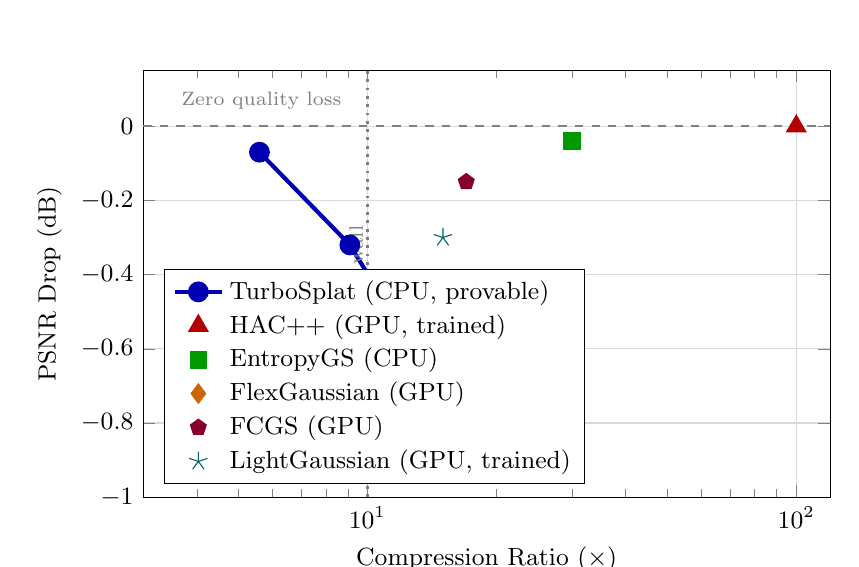
\begin{tikzpicture}
\begin{axis}[
    width=0.85\textwidth,
    height=7cm,
    xlabel={Compression Ratio ($\times$)},
    ylabel={PSNR Drop (dB)},
    xmin=3, xmax=120,
    ymin=-1.0, ymax=0.15,
    xmode=log,
    log basis x={10},
    grid=major,
    grid style={gray!30},
    legend pos=south west,
    legend style={font=\small, cells={anchor=west}},
    every axis label/.style={font=\small},
    every tick label/.style={font=\small},
]
% TurboSplat Pareto
\addplot[
    color=blue!70!black,
    mark=*,
    mark size=3pt,
    line width=1.5pt,
] coordinates {
    (5.6, -0.07)
    (9.1, -0.32)
    (12.5, -0.58)
};
\addlegendentry{\ours{} (CPU, provable)}

% Competitors
\addplot[only marks, mark=triangle*, mark size=4pt, color=red!70!black] coordinates {(100, 0.0)};
\addlegendentry{HAC++ (GPU, trained)}

\addplot[only marks, mark=square*, mark size=3pt, color=green!60!black] coordinates {(30, -0.04)};
\addlegendentry{EntropyGS (CPU)}

\addplot[only marks, mark=diamond*, mark size=3.5pt, color=orange!80!black] coordinates {(20, -0.50)};
\addlegendentry{FlexGaussian (GPU)}

\addplot[only marks, mark=pentagon*, mark size=3pt, color=purple!70!black] coordinates {(17, -0.15)};
\addlegendentry{FCGS (GPU)}

\addplot[only marks, mark=star, mark size=3.5pt, color=teal!80!black] coordinates {(15, -0.30)};
\addlegendentry{LightGaussian (GPU, trained)}

% Free compression threshold
\addplot[gray, dashed, line width=0.8pt] coordinates {(3, 0) (120, 0)};
\node[font=\scriptsize, text=gray, anchor=south west] at (axis cs:3.5, 0.02) {Zero quality loss};

% Quantization wall annotation
\draw[gray, dotted, line width=1pt] (axis cs:10, -1.0) -- (axis cs:10, 0.15);
\node[font=\scriptsize, text=gray, rotate=90, anchor=south] at (axis cs:10.5, -0.5) {Quantization wall};

\end{axis}
\end{tikzpicture}
\caption{\textbf{Rate-distortion frontier of 3DGS compression.} \ours{} (blue curve) traces the frontier of training-free compression with provable optimality guarantees. Competing methods (markers) achieve higher ratios but require GPU access and/or training. The dotted vertical line marks the approximate quantization wall (${\sim}10{\times}$), beyond which training-free methods require Gaussian merging. The dashed horizontal line indicates zero quality loss.}
\Description{Rate-distortion plot comparing TurboSplat to prior 3D Gaussian Splatting compressors. TurboSplat traces a blue curve from a near-lossless low-compression point to a more aggressive operating point near the quantization wall around ten times compression. Competing methods appear as markers at higher compression ratios but rely on GPU processing or training.}
\label{fig:rd_frontier}
\end{figure*}

\begin{figure*}[t]
\centering
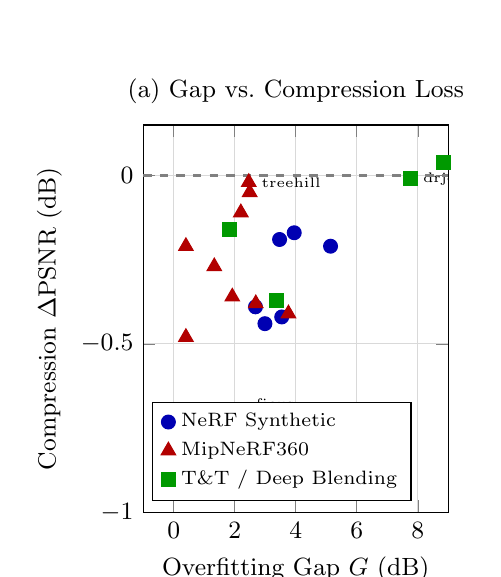
\begin{tikzpicture}
\begin{axis}[
    width=0.45\textwidth,
    height=6.5cm,
    xlabel={Overfitting Gap $G$ (dB)},
    ylabel={Compression $\Delta$PSNR (dB)},
    xmin=-1, xmax=9,
    ymin=-1.0, ymax=0.15,
    grid=major,
    grid style={gray!30},
    every axis label/.style={font=\small},
    every tick label/.style={font=\small},
    title={\small (a) Gap vs.\ Compression Loss},
    title style={yshift=-2pt},
    legend pos=south west,
    legend style={font=\scriptsize, cells={anchor=west}},
]
% NeRF Synthetic scenes (blue circles)
\addplot[only marks, mark=*, mark size=2.5pt, color=blue!70!black] coordinates {
    (3.95, -0.17) (3.54, -0.42) (3.47, -0.19) (3.32, -0.72)
    (2.99, -0.44) (5.14, -0.21) (4.04, -0.90) (2.68, -0.39)
};
\addlegendentry{NeRF Synthetic}

% MipNeRF360 scenes (red triangles)
\addplot[only marks, mark=triangle*, mark size=3pt, color=red!70!black] coordinates {
    (0.40, -0.21) (0.40, -0.48) (1.33, -0.27) (2.20, -0.11)
    (2.49, -0.05) (1.92, -0.36) (2.69, -0.38) (3.76, -0.41) (2.46, -0.02)
};
\addlegendentry{MipNeRF360}

% T&T and DB scenes (green squares)
\addplot[only marks, mark=square*, mark size=2.5pt, color=green!60!black] coordinates {
    (1.84, -0.16) (3.38, -0.37) (7.75, -0.01) (8.84, 0.04)
};
\addlegendentry{T\&T / Deep Blending}

% Labels for notable scenes
\node[font=\tiny, anchor=west] at (axis cs:7.75, -0.01) {\,drjohnson};
\node[font=\tiny, anchor=south west] at (axis cs:8.84, 0.04) {\,playroom};
\node[font=\tiny, anchor=south] at (axis cs:3.32, -0.72) {ficus};
\node[font=\tiny, anchor=south] at (axis cs:4.04, -0.90) {mic};
\node[font=\tiny, anchor=west] at (axis cs:2.46, -0.02) {\,treehill};

% Free compression line
\addplot[gray, dashed, line width=0.8pt] coordinates {(-1, 0) (9, 0)};

\end{axis}
\end{tikzpicture}%
\hfill
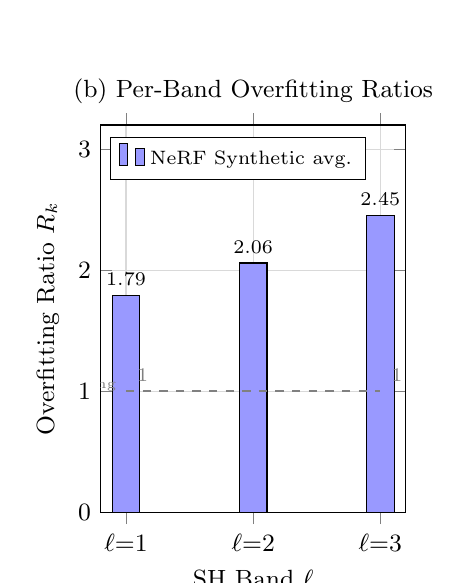
\begin{tikzpicture}
\begin{axis}[
    width=0.45\textwidth,
    height=6.5cm,
    ybar,
    bar width=10pt,
    xlabel={SH Band $\ell$},
    ylabel={Overfitting Ratio $\R{k}$},
    symbolic x coords={$\ell{=}1$, $\ell{=}2$, $\ell{=}3$},
    xtick=data,
    ymin=0, ymax=3.2,
    grid=major,
    grid style={gray!30},
    every axis label/.style={font=\small},
    every tick label/.style={font=\small},
    title={\small (b) Per-Band Overfitting Ratios},
    title style={yshift=-2pt},
    legend pos=north west,
    legend style={font=\scriptsize},
    nodes near coords,
    every node near coord/.append style={font=\scriptsize},
    nodes near coords style={/pgf/number format/.cd, fixed, precision=2},
]
\addplot[fill=blue!40!white] coordinates {
    ($\ell{=}1$, 1.79)
    ($\ell{=}2$, 2.06)
    ($\ell{=}3$, 2.45)
};
\addlegendentry{NeRF Synthetic avg.}

% Reference line at R=1
\addplot[gray, dashed, line width=0.6pt, sharp plot, forget plot] coordinates {
    ($\ell{=}1$, 1.0)
    ($\ell{=}3$, 1.0)
};

\node[font=\tiny, text=gray, anchor=east] at (axis cs: $\ell{=}1$, 1.05) {No overfitting};

\end{axis}
\end{tikzpicture}
\caption{\textbf{SH overfitting analysis.} (a)~Overfitting gap $G$ versus compression-induced PSNR change for all 21 scenes. Scenes with large or destructive overfitting (drjohnson, playroom, treehill) lie near zero compression loss, whereas scenes with genuine view-dependent content (mic, ficus) incur larger losses. (b)~Average overfitting ratio $\R{k}$ per SH band on NeRF Synthetic, showing the consistent hierarchy $\R{1} < \R{2} < \R{3}$. The dashed line at $\R{k}{=}1$ indicates zero overfitting; $\R{3}{=}2.45$ implies ${\sim}59\%$ of band~3 content is noise.}
\Description{Two-panel figure. The left panel is a scatter plot of overfitting gap versus compression-induced PSNR change for all scenes; high-gap scenes such as playroom and drjohnson lie close to zero loss, while mic and ficus incur the largest losses. The right panel is a bar chart of average NeRF Synthetic overfitting ratios by spherical harmonic band, increasing from R1 to R3 and showing the strongest overfitting in band three.}
\label{fig:overfitting}
\end{figure*}

\begin{figure*}[t]
\centering
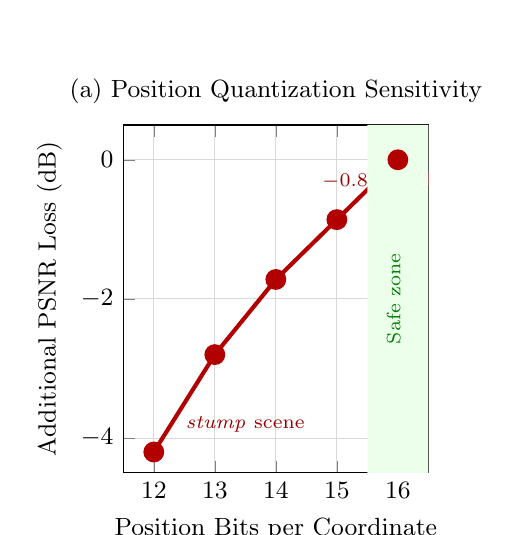
\begin{tikzpicture}
\begin{axis}[
    width=0.45\textwidth,
    height=6cm,
    xlabel={Position Bits per Coordinate},
    ylabel={Additional PSNR Loss (dB)},
    xmin=11.5, xmax=16.5,
    ymin=-4.5, ymax=0.5,
    xtick={12,13,14,15,16},
    grid=major,
    grid style={gray!30},
    every axis label/.style={font=\small},
    every tick label/.style={font=\small},
    title={\small (a) Position Quantization Sensitivity},
    title style={yshift=-2pt},
]
\addplot[
    color=red!70!black,
    mark=*,
    mark size=3pt,
    line width=1.5pt,
] coordinates {
    (16, 0)
    (15, -0.86)
    (14, -1.72)
    (13, -2.80)
    (12, -4.20)
};

\node[font=\scriptsize, anchor=south west, text=red!60!black] at (axis cs:14.6, -0.6) {$-$0.86 dB/bit};

% Safe zone shading
\addplot[fill=green!8, draw=none, forget plot] coordinates {(15.5, 0.5) (16.5, 0.5) (16.5, -4.5) (15.5, -4.5)} \closedcycle;
\node[font=\scriptsize, text=green!50!black, rotate=90, anchor=south] at (axis cs:16.2, -2.0) {Safe zone};

% Danger zone label
\node[font=\scriptsize, text=red!60!black] at (axis cs:13.5, -3.8) {\textit{stump} scene};

\end{axis}
\end{tikzpicture}%
\hfill
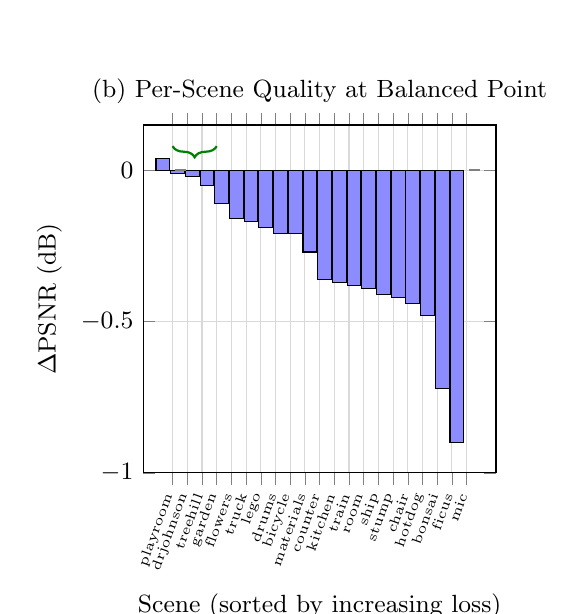
\begin{tikzpicture}
\begin{axis}[
    width=0.50\textwidth,
    height=6cm,
    ybar,
    bar width=5pt,
    xlabel={Scene (sorted by increasing loss)},
    ylabel={$\Delta$PSNR (dB)},
    symbolic x coords={playroom,drjohnson,treehill,garden,flowers,truck,lego,drums,bicycle,materials,counter,kitchen,train,room,ship,stump,chair,hotdog,bonsai,ficus,mic},
    xtick=data,
    x tick label style={rotate=70, anchor=east, font=\tiny},
    ymin=-1.0, ymax=0.15,
    grid=major,
    grid style={gray!30},
    every axis label/.style={font=\small},
    every tick label/.style={font=\small},
    title={\small (b) Per-Scene Quality at Balanced Point},
    title style={yshift=-2pt},
]
\addplot[fill=blue!45!white] coordinates {
    (playroom, 0.04)
    (drjohnson, -0.01)
    (treehill, -0.02)
    (garden, -0.05)
    (flowers, -0.11)
    (truck, -0.16)
    (lego, -0.17)
    (drums, -0.19)
    (bicycle, -0.21)
    (materials, -0.21)
    (counter, -0.27)
    (kitchen, -0.36)
    (train, -0.37)
    (room, -0.38)
    (ship, -0.39)
    (stump, -0.41)
    (chair, -0.42)
    (hotdog, -0.44)
    (bonsai, -0.48)
    (ficus, -0.72)
    (mic, -0.90)
};

% Free compression line
\addplot[gray, dashed, line width=0.8pt] coordinates {(playroom, 0) (mic, 0)};

% Bracket for free compression
\draw[decorate, decoration={brace, amplitude=4pt, mirror}, thick, green!50!black]
    (axis cs:playroom, 0.08) -- (axis cs:garden, 0.08)
    node[midway, above, yshift=4pt, font=\tiny, text=green!50!black] {Free ($<$0.05 dB)};

\end{axis}
\end{tikzpicture}
\caption{\textbf{Quantization wall and per-scene results.} (a)~Position bit sensitivity on \textit{stump}: each bit removed below 16 incurs ${\sim}0.86\dB$ additional loss, establishing 16-bit positions as the minimum for COLMAP scenes. This sensitivity defines the quantization wall for training-free compression. (b)~Per-scene PSNR change at the balanced operating point ($9.1{\times}$ average), sorted by increasing loss. Four scenes (playroom, drjohnson, treehill, garden) achieve effectively free compression; playroom \emph{improves} under compression.}
\Description{Two-panel figure. The left panel plots additional PSNR loss versus position-bit precision on the stump scene and shows rapidly increasing degradation below sixteen bits, highlighting a quantization wall. The right panel is a bar chart of per-scene PSNR change at the balanced compression point; playroom, drjohnson, treehill, and garden are closest to zero loss, while mic and ficus have the largest losses.}
\label{fig:wall}
\end{figure*}

\begin{figure*}[t]
\centering
\begin{tabular}{@{}c@{\hspace{2pt}}c@{\hspace{2pt}}c@{}}
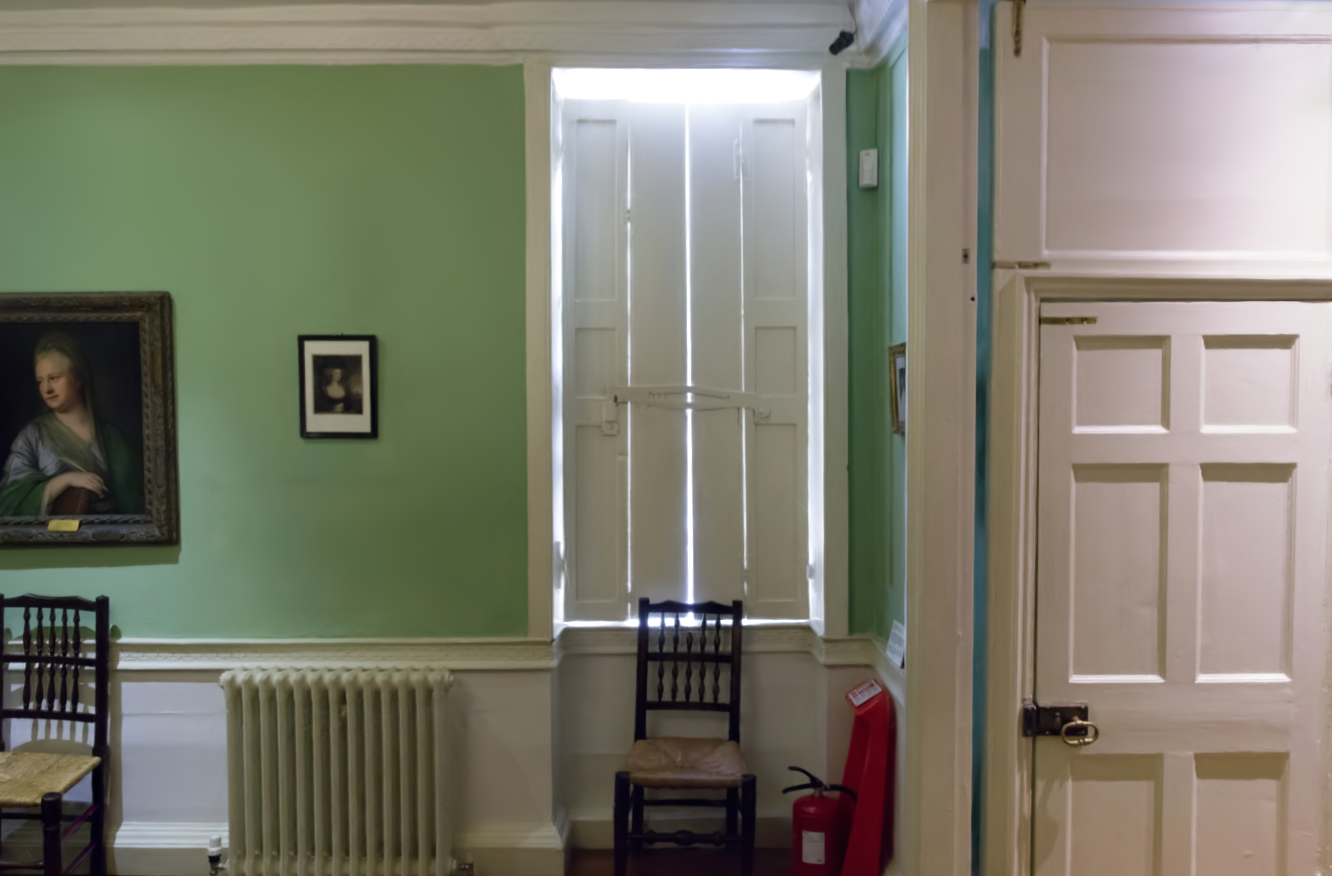
\includegraphics[width=0.325\textwidth]{figures/renders/drjohnson_original.png} &
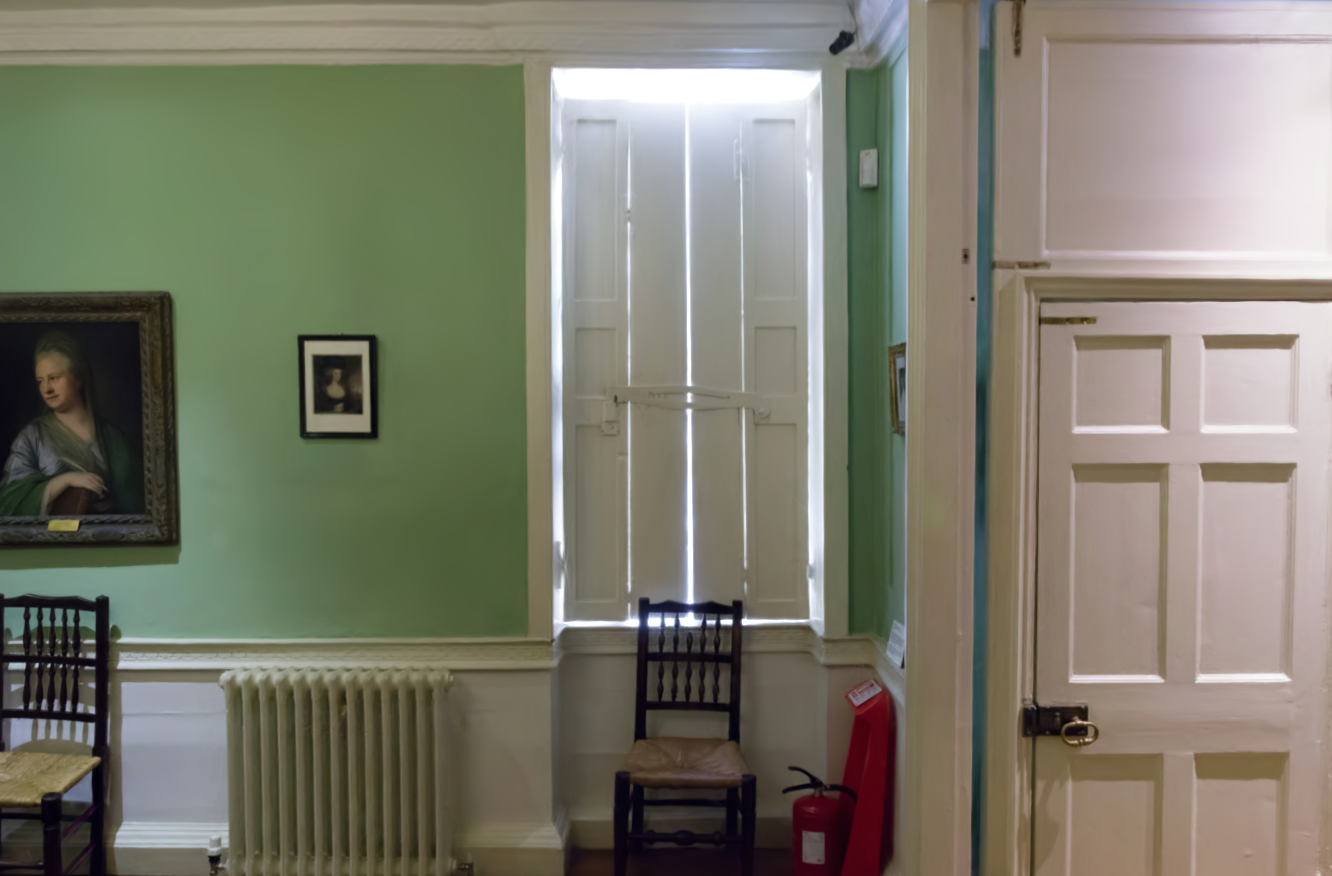
\includegraphics[width=0.325\textwidth]{figures/renders/drjohnson_compressed.png} &
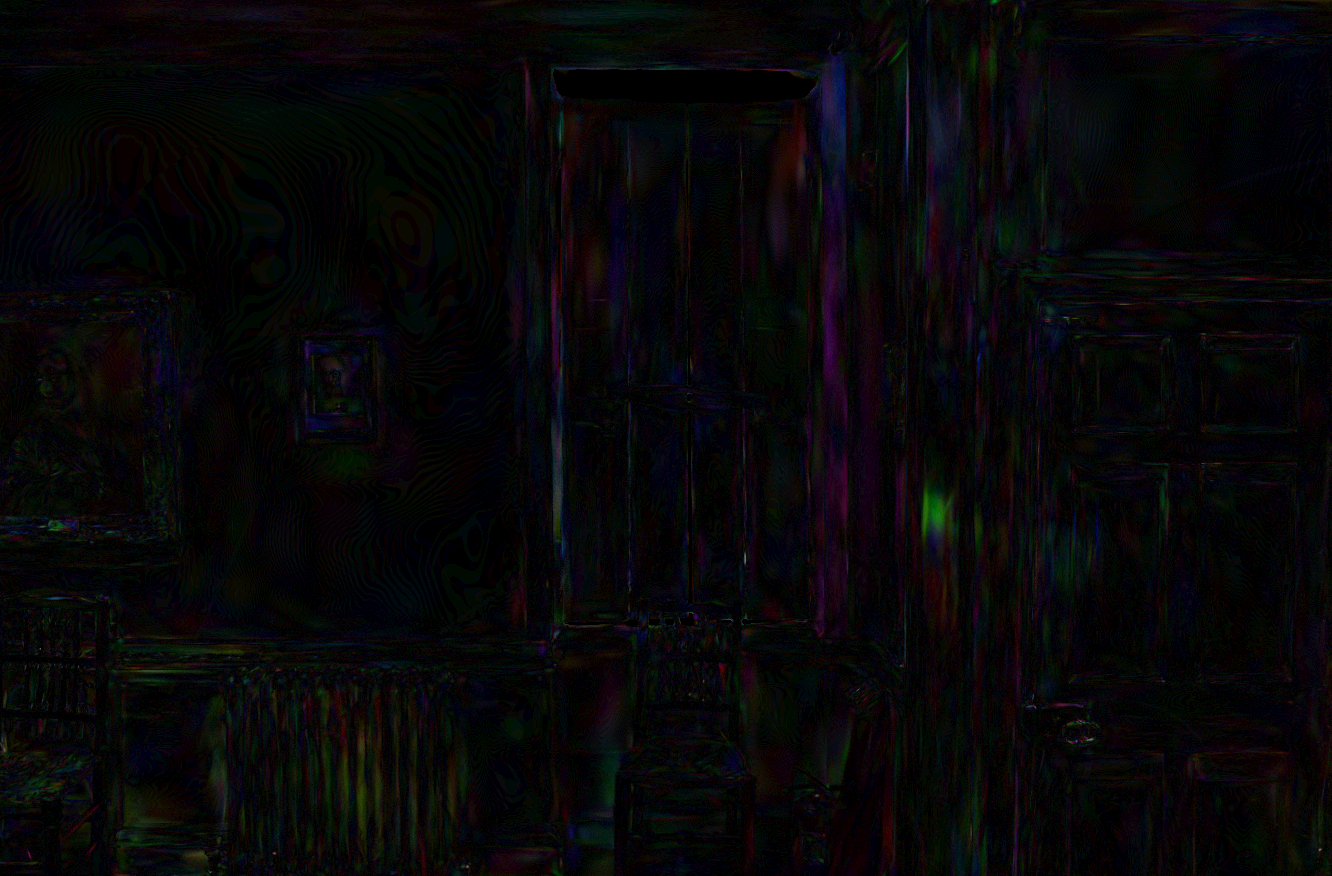
\includegraphics[width=0.325\textwidth]{figures/renders/drjohnson_error_10x.png} \\
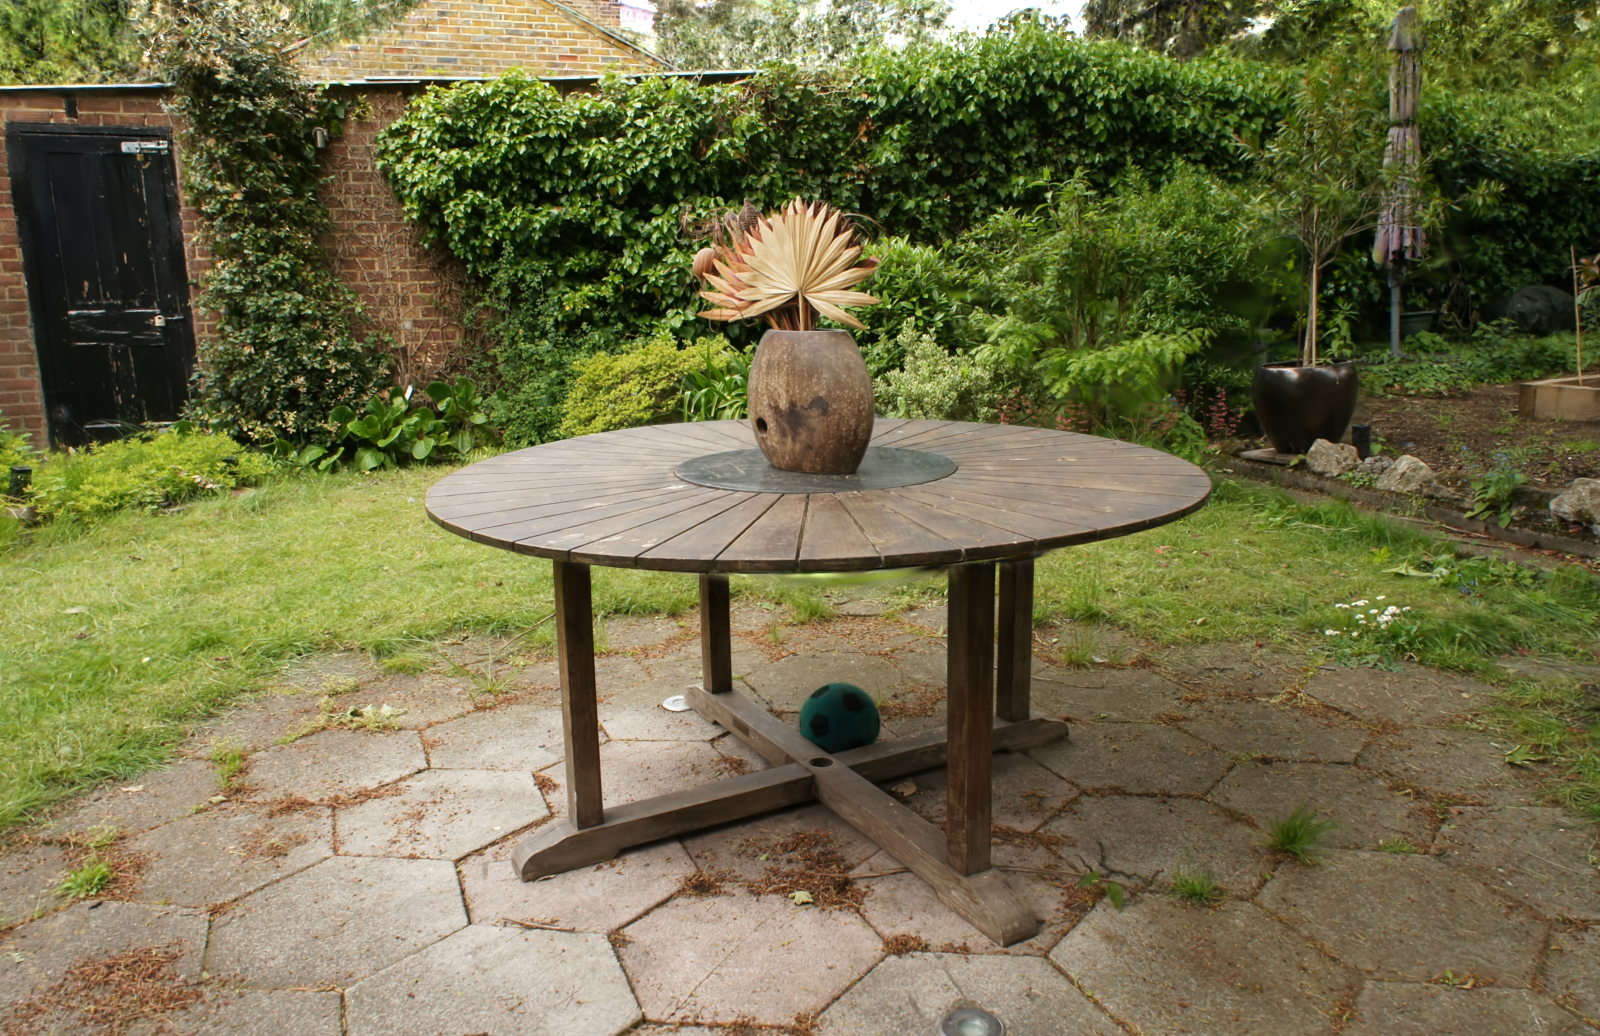
\includegraphics[width=0.325\textwidth]{figures/renders/garden_original.png} &
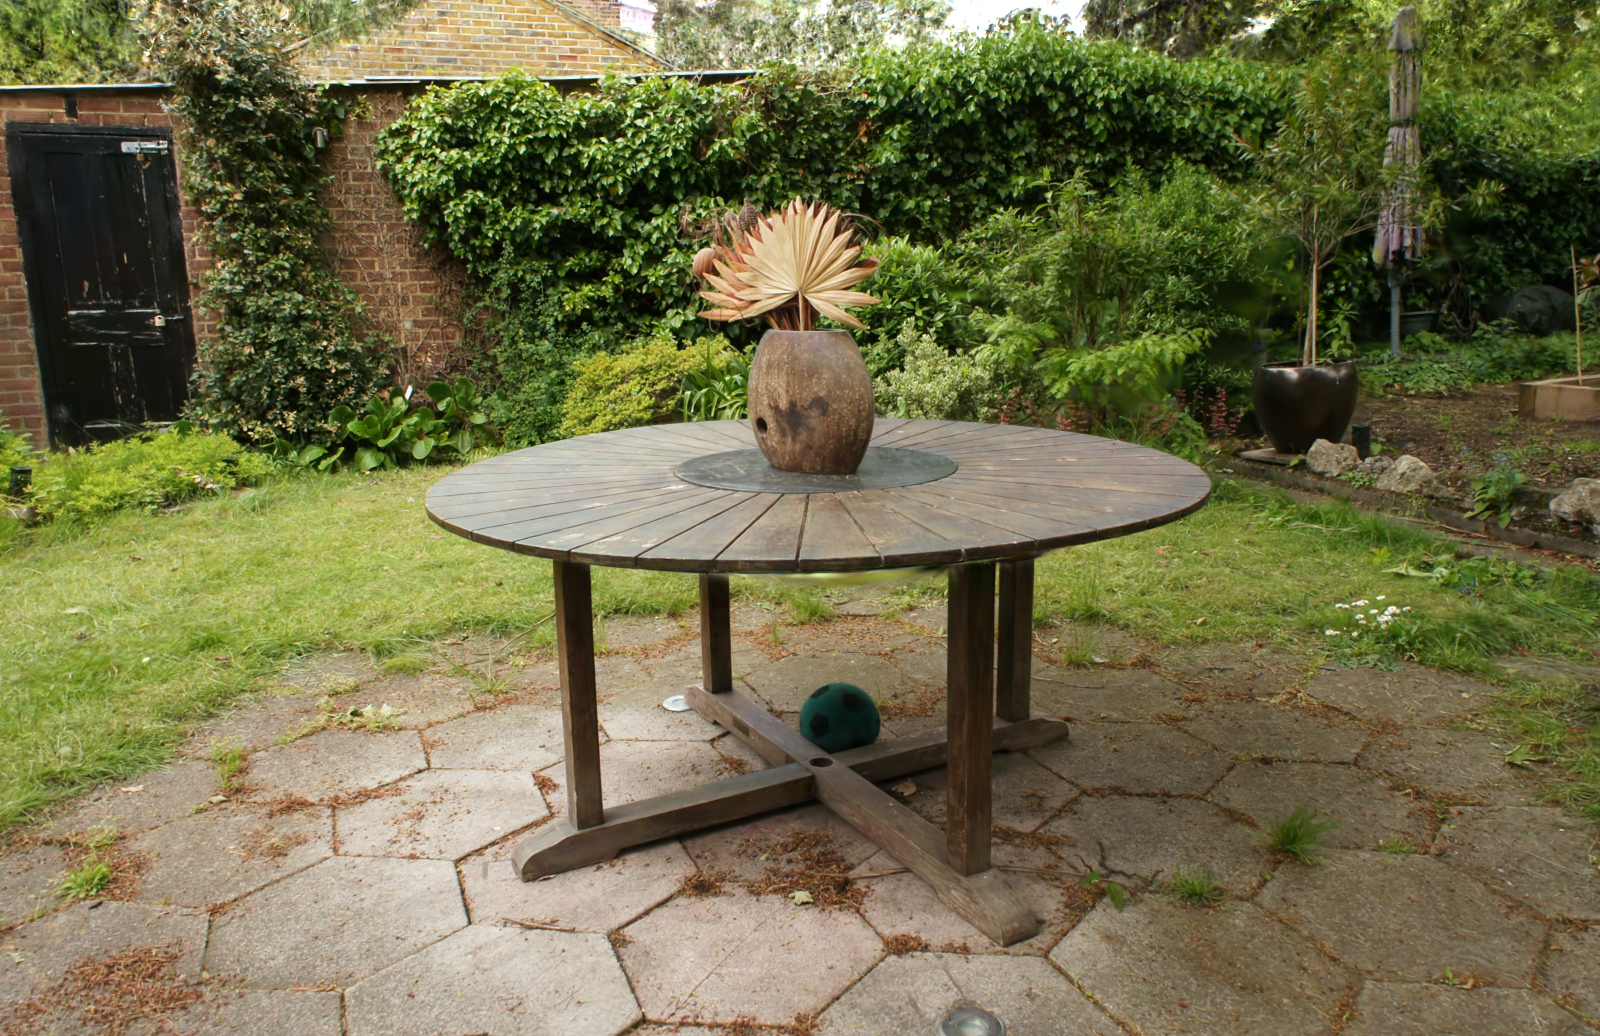
\includegraphics[width=0.325\textwidth]{figures/renders/garden_compressed.png} &
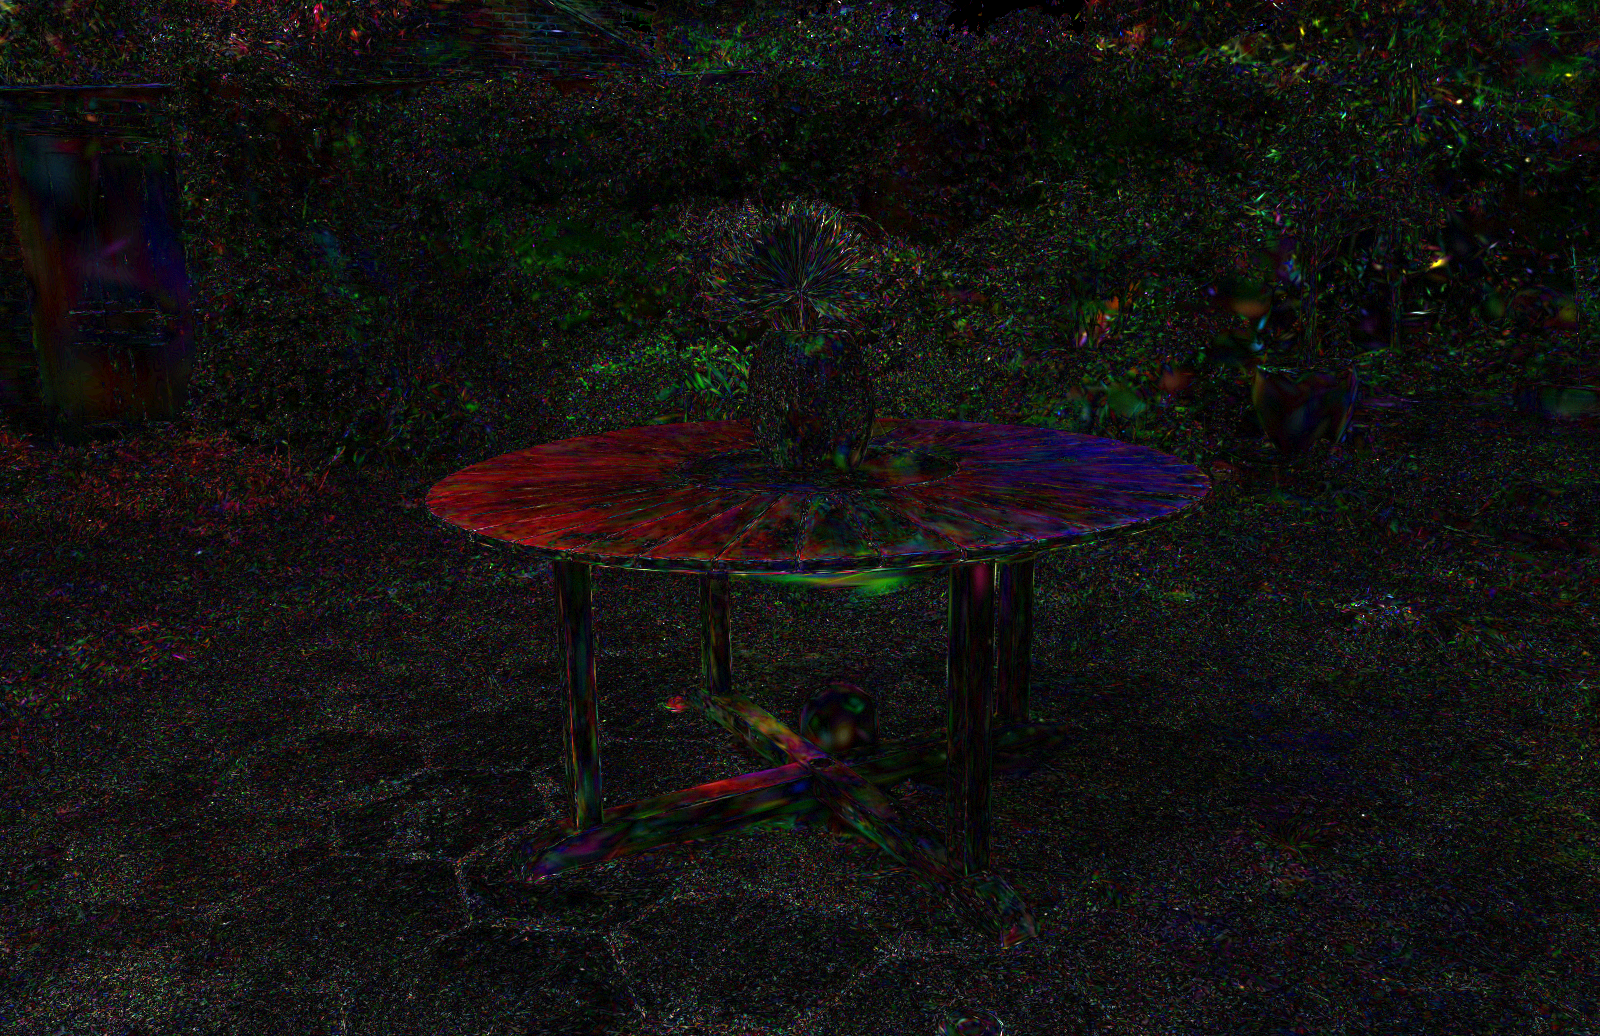
\includegraphics[width=0.325\textwidth]{figures/renders/garden_error_10x.png} \\
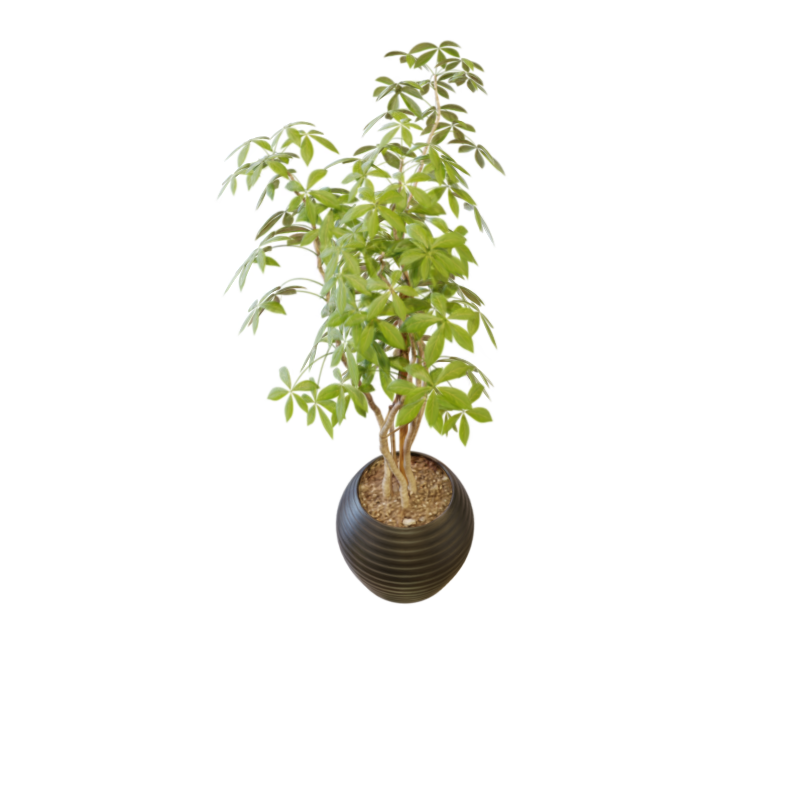
\includegraphics[width=0.325\textwidth]{figures/renders/ficus_original.png} &
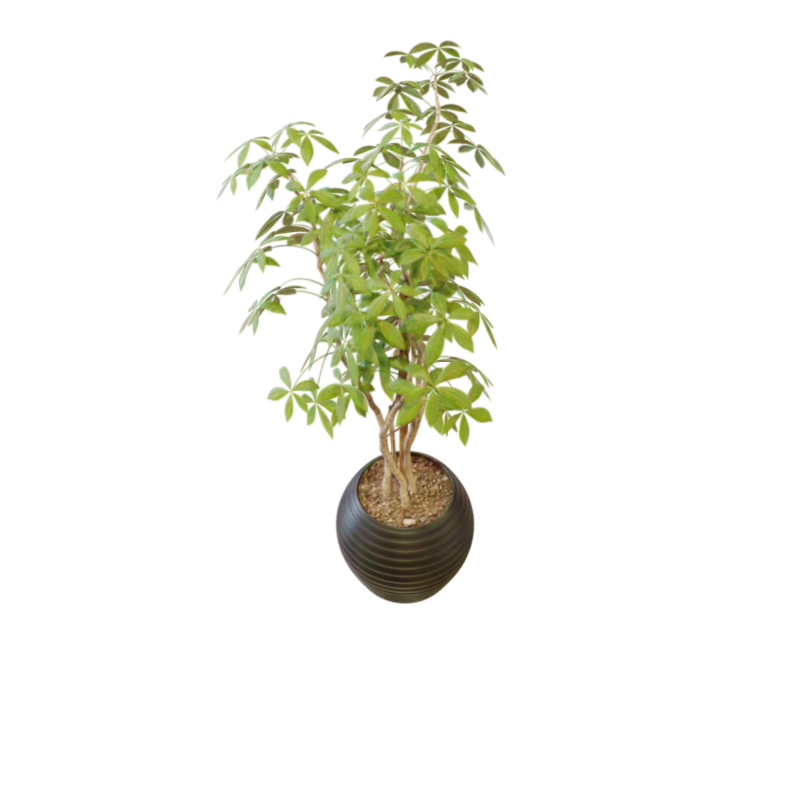
\includegraphics[width=0.325\textwidth]{figures/renders/ficus_compressed.png} &
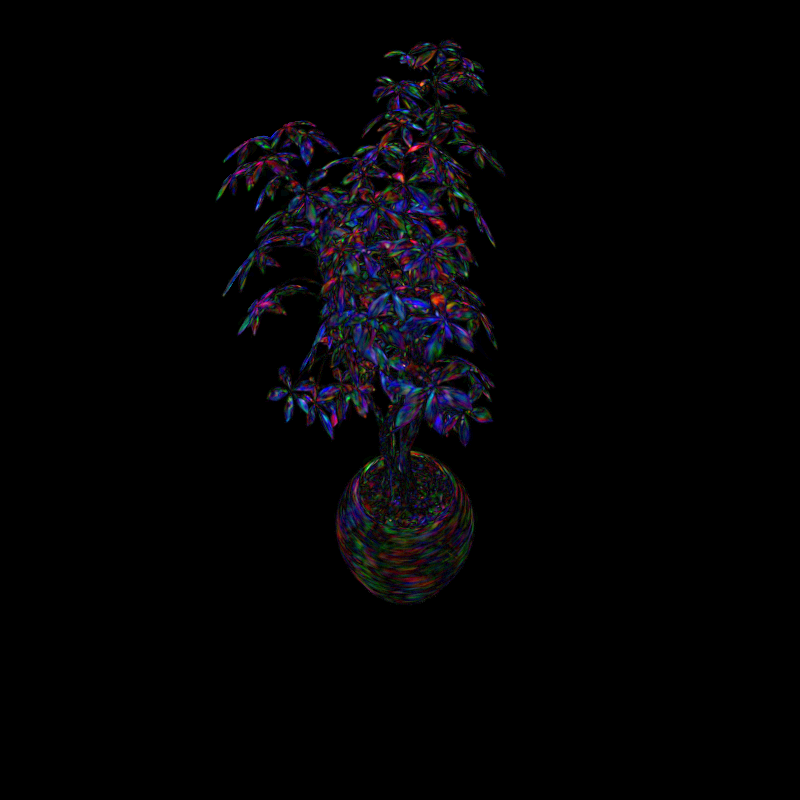
\includegraphics[width=0.325\textwidth]{figures/renders/ficus_error_10x.png} \\
{\small Original} & {\small \ours{} Compressed} & {\small Error $\times$10} \\
\end{tabular}
\caption{\textbf{Visual quality comparison at $9.1{\times}$ average compression.} Left: original render. Center: \ours{} compressed. Right: error map (amplified $10{\times}$). \textit{drjohnson} (top) shows no visible difference at $0.01\dB$ loss. \textit{garden} (middle) incurs $0.05\dB$ loss. \textit{ficus} (bottom) is the worst case at $0.72\dB$, with visible artifacts on fine leaf structures.}
\Description{Three rows of render comparisons. Each row shows the original rendering, the TurboSplat-compressed rendering, and a ten-times-amplified error map for one scene. drjohnson shows almost no visible difference, garden shows very small differences, and ficus shows the clearest artifacts on fine leaves and view-dependent detail.}
\label{fig:renders}
\end{figure*}

%% ============================================================
%% REFERENCES
%% ============================================================
\bibliographystyle{ACM-Reference-Format}
\bibliography{references}

\end{document}
